\documentclass{article}
\usepackage{graphicx}
\usepackage{subcaption}
\usepackage{amsmath}
\usepackage{cite}

\title{Study of the Melting of a Lennard-Jones FCC Crystal}
\author{ALESSANDRO CROTTI}
\date{April 2025}

\begin{document}

\maketitle

\section{Introduction}

Melting is the phase transition of a substance from an ordered solid to a disordered liquid state. This process involves increasing the internal energy of the solid, causing its atoms to break free from the rigid crystal lattice and move more freely. For a pure substance, this transition ideally occurs at a sharp, well-defined melting point.

In this project, we investigate the melting process of a bulk Lennard-Jones (LJ) crystal with a face-centered cubic (FCC) structure using molecular dynamics (MD) simulations. The LJ potential is a simple yet realistic model for the interactions between neutral atoms, making it a cornerstone of computational physics. It is defined as:
$$V_{LJ}(r) = 4\epsilon\left[\left(\frac{\sigma}{r}\right)^{12} - \left(\frac{\sigma}{r}\right)^6\right]$$
where $\epsilon$ is the depth of the potential well and $\sigma$ is the finite distance at which the potential is zero.

Our goal is to characterize the solid-to-liquid transition by monitoring a suite of thermodynamic, structural, and dynamical observables. We will analyze how quantities such as energy, density, mean-square displacement (MSD), and the radial distribution function ($g(r)$) evolve with temperature. Furthermore, we will investigate the role of kinetic effects, such as superheating, by studying the system's response to different heating rates, thereby distinguishing between the observed melting behavior and the true thermodynamic transition.

\section{Simulation Methodology}

The molecular dynamics (MD) simulations were performed using the \verb|LAMMPS| software package \cite{LAMMPS}. Trajectory visualization was done with \verb|VMD| \cite{VMD}, and data analysis was carried out using custom scripts in \verb|MATLAB|.

\subsection{System Setup}

The simulation environment was defined using LJ units, where energy is measured in units of $\epsilon$, distance in $\sigma$, and mass in units of the particle mass $m$. The simulation box was configured with periodic boundary conditions in all three dimensions to model a bulk system.

An FCC lattice was created with a lattice constant of 1.122, which is close to the equilibrium spacing. The unit cell was replicated $10 \times 10 \times 10$ times to create a supercell containing $N=4000$ atoms. Initial velocities were assigned from a Maxwell-Boltzmann distribution at $T^* = 0.3$. The 12-6 LJ pair potential was employed with a cutoff radius of $r_c = 2.5\sigma$, shifted to ensure the potential is zero at the cutoff.

\subsection{Equilibration and Simulation Protocol}

A crucial first step is to bring the system to thermal equilibrium. The system was evolved under an NPT ensemble (constant number of particles, pressure, and temperature) at $T^*=0.3$ and $P^*=0$. To determine the necessary equilibration time, the system's potential energy and temperature were monitored (\textbf{Figure \ref{fig:equilibration}}). Both quantities stabilized after approximately $15,000$ steps. A conservative equilibration period of $50,000$ steps was chosen for our production runs.

\begin{figure}[htbp]
    \centering
    \begin{subfigure}[b]{0.49\textwidth}
        \centering
        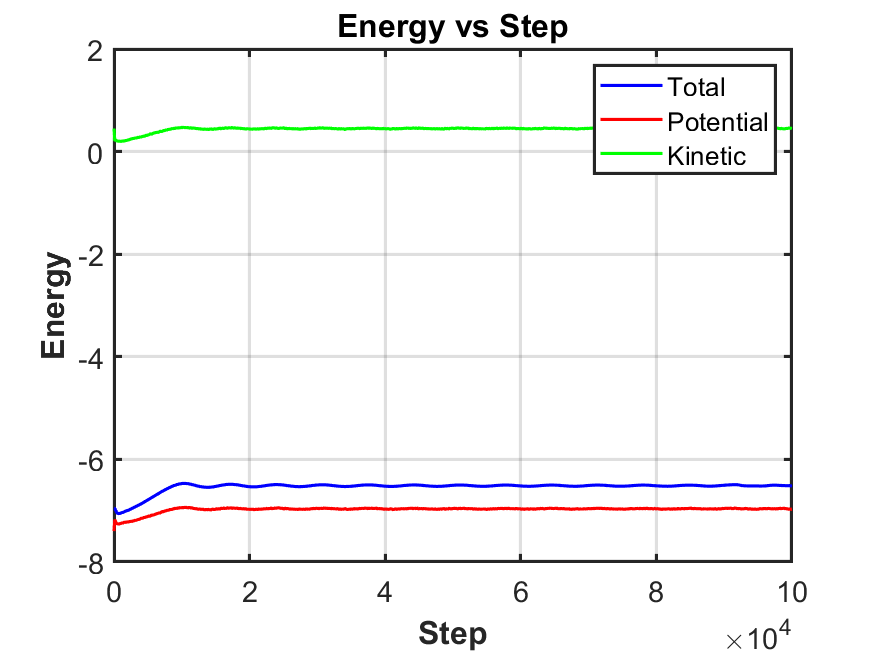
\includegraphics[width=\linewidth]{energies_vs_step_50000.png}
        \caption{Evolution of energies during equilibration.}
        \label{fig:equil_energy}
    \end{subfigure}
    \hfill
    \begin{subfigure}[b]{0.49\textwidth}
        \centering
        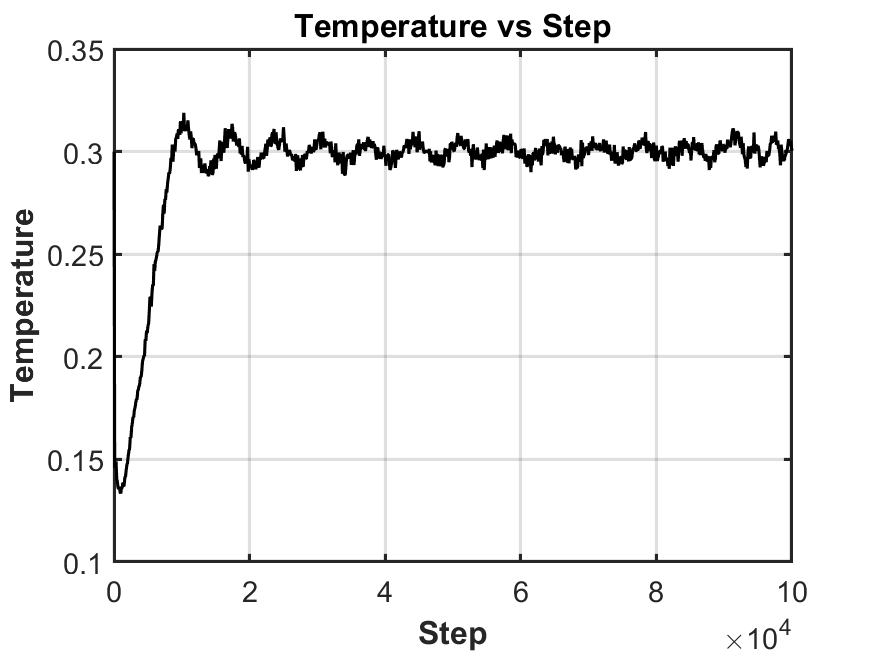
\includegraphics[width=\linewidth]{temperature_vs_step_50000.png}
        \caption{Evolution of temperature during equilibration.}
        \label{fig:equil_temp}
    \end{subfigure}
    \caption{System equilibration at $T^*=0.3$. The system reaches a stable steady-state after approximately $15,000$ steps.}
    \label{fig:equilibration}
\end{figure}

The primary simulation protocol consisted of three stages, all using a timestep of $0.005\tau$:
\begin{enumerate}
    \item \textbf{Initial Equilibration:} $50,000$ steps at $T^*=0.3$ and $P^*=0$.
    \item \textbf{Heating Ramp:} $80,000$ steps where the temperature was ramped linearly from $T^*=0.3$ to $T^*=2.0$ at $P^*=0$ which is the more accurate result as you can see in \textbf{Fig. \ref{fig:heating_rates}}
    \item \textbf{Final Equilibration:} $50,000$ steps at the final temperature of $T^*=2.0$.
\end{enumerate}
The NPT ensemble was chosen to allow the simulation box to expand or contract in response to temperature changes at constant zero pressure. This was implemented using a Nosé-Hoover thermostat and barostat \cite{Nose, Hoover}, which maintains the target temperature and pressure by coupling the system to external reservoirs.


A timestep of $\Delta t = 0.005\,\tau$ was selected for the simulations. In the NPT ensemble, the total energy of the system is not a conserved quantity due to the necessary energy exchange with the external heat bath and barostat, as managed by the Nosé-Hoover algorithm \cite{Nose, Hoover}. Therefore, the suitability of the chosen timestep is not validated by checking for strict energy conservation, but rather by ensuring the stability of the integrator and observing physically meaningful fluctuations.

To this end, the total energy was monitored during the initial equilibration phase at $T^*=0.3$. As shown in \textbf{Figure \ref{fig:npt_energy_equilibration}}, after an initial transient period of approximately 15,000 steps, the system settles into a stable steady-state. In this regime, the energy oscillates around a well-defined mean value without any systematic long-term drift, which confirms the stability of the numerical integration.

\begin{figure}[htbp]
    \centering
    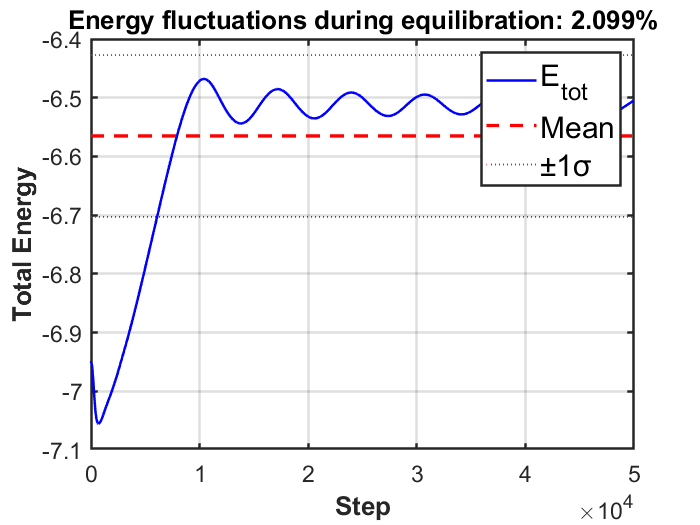
\includegraphics[width=0.9\linewidth]{uncertanty.png}
    \caption{Evolution of the total energy per particle during the initial NPT equilibration at $T^*=0.3$. The system reaches a stable steady-state, oscillating around a constant mean value. The magnitude of these fluctuations is a physical property of the system, related to its heat capacity.}
    \label{fig:npt_energy_equilibration}
\end{figure}

A quantitative analysis of the equilibrated portion of the trajectory (from step $15\ 000$ to $50\ 000$) yields a mean total energy $\langle E \rangle = -6.5651\,\epsilon$ with a standard deviation of $\sigma_E = 0.1378\,\epsilon$. The resulting relative fluctuation, calculated as $\sigma_E/|\langle E \rangle|$, is approximately 2.099\%. This magnitude of fluctuation is not an artifact of the integration but a fundamental physical characteristic of the canonical ensemble. According to statistical mechanics, the variance of the energy is directly proportional to the system's heat capacity \cite{AllenTildesley}. The observed stability, coupled with a fluctuation level that is physically reasonable for an NPT simulation, confirms that the chosen timestep of $0.005\,\tau$ is appropriate for accurately sampling the system's dynamics. 


\subsection{Qualitative Visualization}

To obtain a qualitative picture of the melting process, we rendered the simulation trajectory with VMD. Three representative snapshots are displayed in \textbf{Figure \ref{fig:vmd_snapshots}}. \textbf{Figure \ref{fig:solid}} shows the perfectly ordered solid at low temperature ($T=0.3\frac{\epsilon}{kB}$). \textbf{Figure \ref{fig:melting}} captures the system mid-transition, with coexisting crystalline and disordered regions. Finally ($T\approx0.8\frac{\epsilon}{kB}$), \textbf{Figure \ref{fig:liquid}} depicts the fully disordered liquid state at high temperature, where the simulation box has visibly expanded ($T=2.0\frac{\epsilon}{kB}$).

\begin{figure}[h!]
    \centering
    \begin{subfigure}{.3\textwidth}
        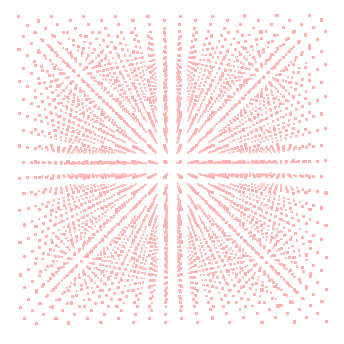
\includegraphics[width=\linewidth]{solid.png}
        \caption{Solid phase \\($T^*=0.3$).}
        \label{fig:solid}
    \end{subfigure}
    \begin{subfigure}{.3\textwidth}
        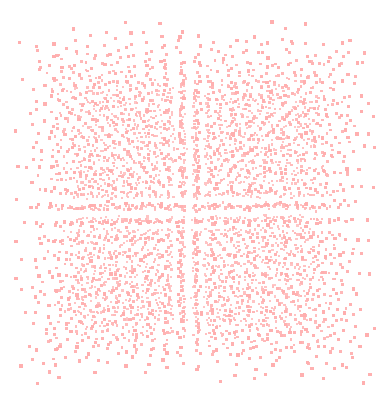
\includegraphics[width=\linewidth]{melting.png}
        \caption{Melting phase \\($T^* \approx 0.8$).}
        \label{fig:melting}
    \end{subfigure}
    \begin{subfigure}{.3\textwidth}
        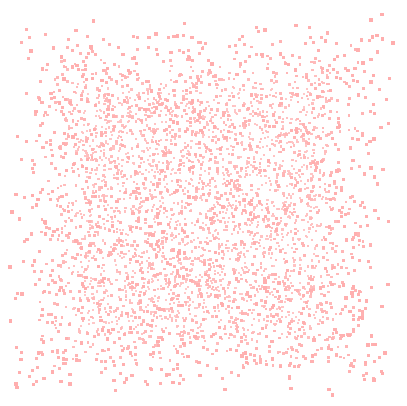
\includegraphics[width=\linewidth]{liquid.png}
        \caption{Liquid phase \\($T^*=2.0$).}
        \label{fig:liquid}
    \end{subfigure}
    \caption{VMD visualizations of the system at different stages of the simulation, showing the transition from an ordered solid to a disordered liquid.}
    \label{fig:vmd_snapshots}
\end{figure}

\section{Results and Analysis}

We analyzed several observables to characterize the melting transition.

\subsection{Thermodynamic Signatures of Melting}

The first-order nature of melting is clearly revealed by the system's thermodynamic properties. In \textbf{Figure \ref{fig:pot_tot_vs_temp}}, the potential and total energies are plotted against temperature. From $T^* \approx 0.3$ to $0.75$, the energy rises smoothly as the solid is heated. Around $T^* \approx 0.8$, a distinct "kink" appears, where the slope of the energy curve increases. This kink signifies the absorption of latent heat of fusion during the phase transition.

\begin{figure}[h!]
    \centering
    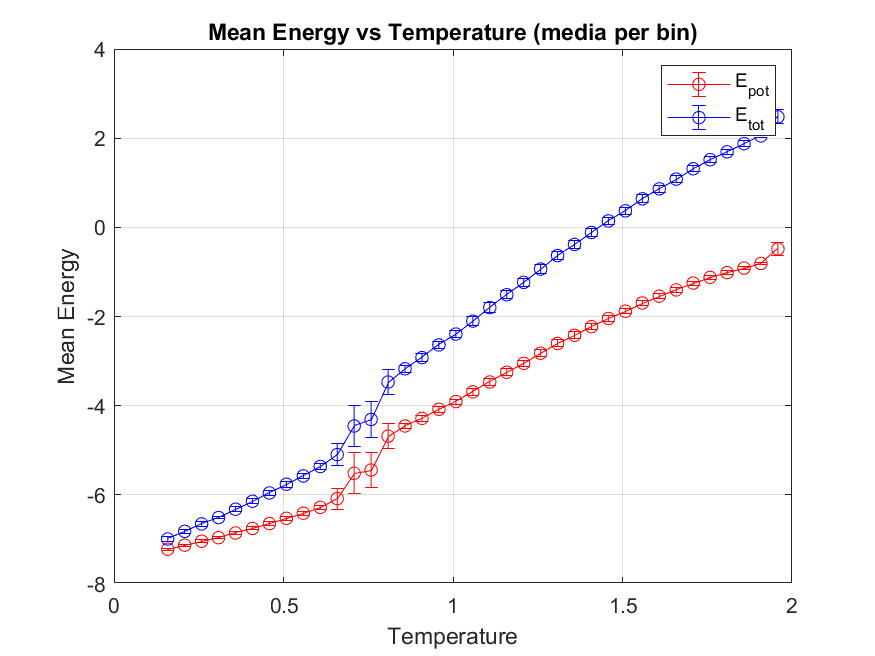
\includegraphics[width=0.7\textwidth]{pot_tot_vs_temp.png}
    \caption{Average potential and total energy vs. temperature. The kink around $T^* \approx 0.8$ indicates the melting transition.}
    \label{fig:pot_tot_vs_temp}
\end{figure}

This is corroborated by \textbf{Figure \ref{fig:tot_temp_vs_step}}, which plots temperature against simulation steps during the heating ramp.
Temperature is a scalar state variable. In our case, temperature is programmed as linear Nose-Hoover ramp from $T\approx0.3$ to $T\approx2.0$. It provides the control parameters for the heating process. 
In \textbf{Fig. \ref{fig:tot_temp_vs_step}}, the curve rises almost lineraly until $T\approx0.8$, where it temporarily plateaus. This plateau occurs as the energy being supplied to the system is used to break the crystal bonds (latent heat) rather than increasing the kinetic energy of the atoms. This plateau is a first-order transition in a driven simulation. Once the system has fully melted, the temperature resumes its linear climb.

\begin{figure}[h!]
    \centering
    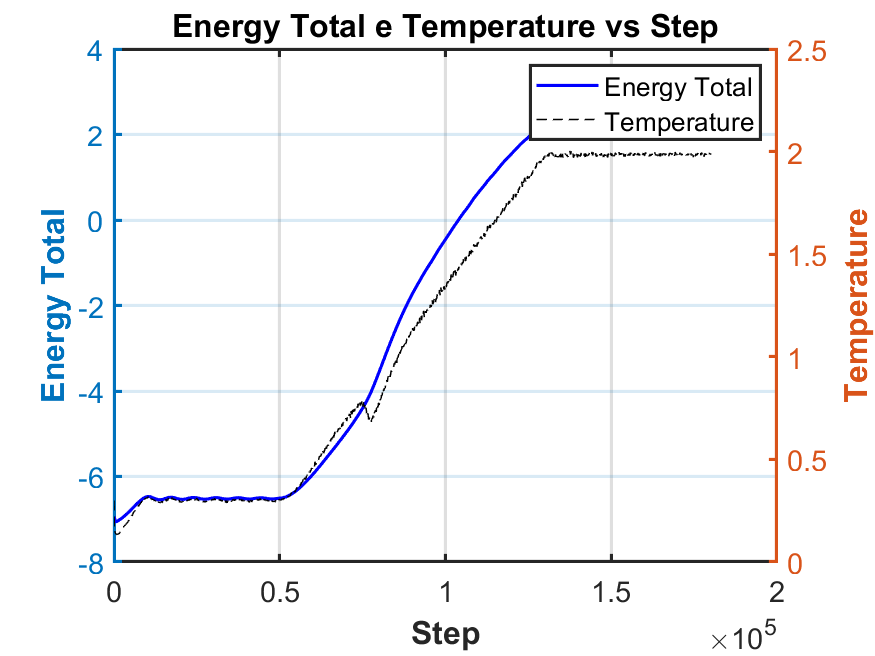
\includegraphics[width=0.7\textwidth]{totenergy_temperature_vs_step.png}
    \caption{Instantaneous total energy and temperature vs. MD step during the simulation. The plateau in temperature around $T^* \approx 0.8$ is a clear signature of a first-order transition.}
    \label{fig:tot_temp_vs_step}
\end{figure}

\subsection{Density}

The mass density is defined as $\rho = Nm/V$, where $N$ is the number of atoms and $V$ is the volume. In LJ reduced units, this is expressed as the number density $\rho^* = N\sigma^3/V$. FCC crystals possess a well-defined equilibrium density at each temperature; melting involves a discontinuous drop in $\rho$ due to volume expansion. 

In \textbf{Fig. \ref{fig:density_vs_temp}}, the density $\rho^*$ is plotted against temperature. The system starts at a high density of $\rho^* \approx 1.05$. As temperature increases, the density decreases smoothly due to thermal expansion. In the region around $T^* \approx 0.8$, the curve exhibits a pronounced drop, which we identify with the solid-liquid phase transition. A key feature is the significant increase in the size of the error bars at the transition point, a hallmark of a first-order phase transition reflecting large density fluctuations. Beyond the transition, the density continues to decrease monotonically.

\begin{figure}[h!]
    \centering
    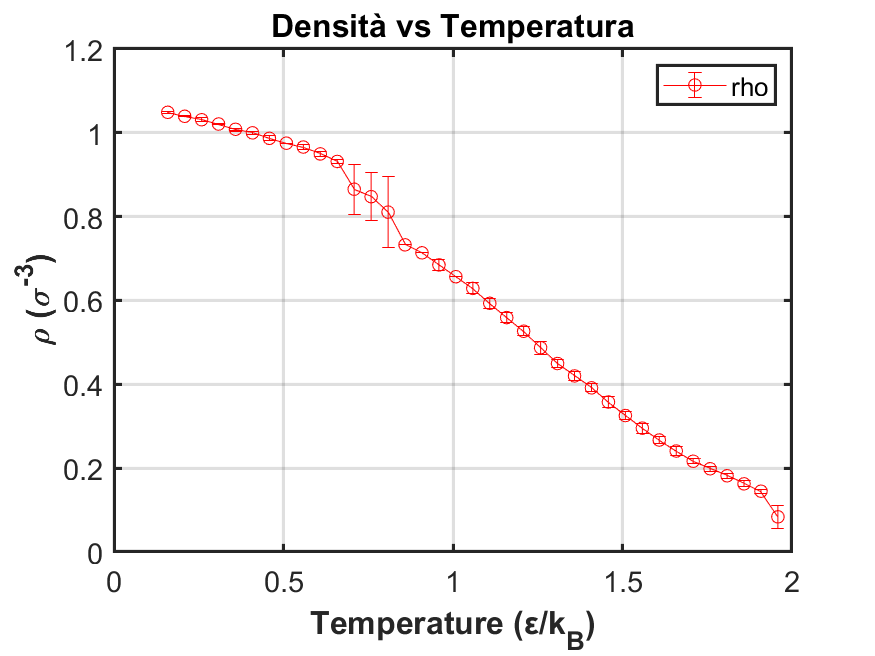
\includegraphics[width=0.7\textwidth]{Fig_Density_T_mean.png}
    \caption{Density $\rho^*$ as a function of temperature $T^*$. The sharp drop around $T^* \approx 0.8$, accompanied by large error bars, signals the melting transition.}
    \label{fig:density_vs_temp}
\end{figure}

\subsection{Mean Square Displacement}

The mean square displacement (MSD) provides insight into the atomic dynamics and is defined as:
$$
\langle\Delta r^2(t)\rangle = \frac{1}{N}\sum_{i=1}^N \langle|\mathbf{r}_i(t) - \mathbf{r}_i(0)|^2\rangle
$$
In a perfect crystal, the MSD plateaus at long times as atoms vibrate around fixed lattice sites. In a liquid, it grows linearly with time, $\langle\Delta r^2(t)\rangle \approx 6Dt$, where $D$ is the self-diffusion coefficient. The crossover from a plateau to diffusive growth provides an unambiguous dynamical criterion for melting.

In \textbf{Fig. \ref{fig:msd_vs_temp}}, we plot the final MSD value against temperature. At low temperatures (up to $T^* \approx 1.2$), the MSD remains close to zero, confirming that atoms are confined to their lattice positions. While the structural transition occurs around $T^* \approx 0.8$, the MSD only begins to show significant growth at higher temperatures. This apparent delay is a physical effect: just above the melting point, the system forms a dense, viscous liquid where diffusion is slow. A large MSD value is only registered at higher temperatures ($T^* > 1.4$), where the liquid is more fluid. The explosive growth of the MSD unambiguously demonstrates the transition to a diffusive liquid state.

\begin{figure}[h!]
    \centering
    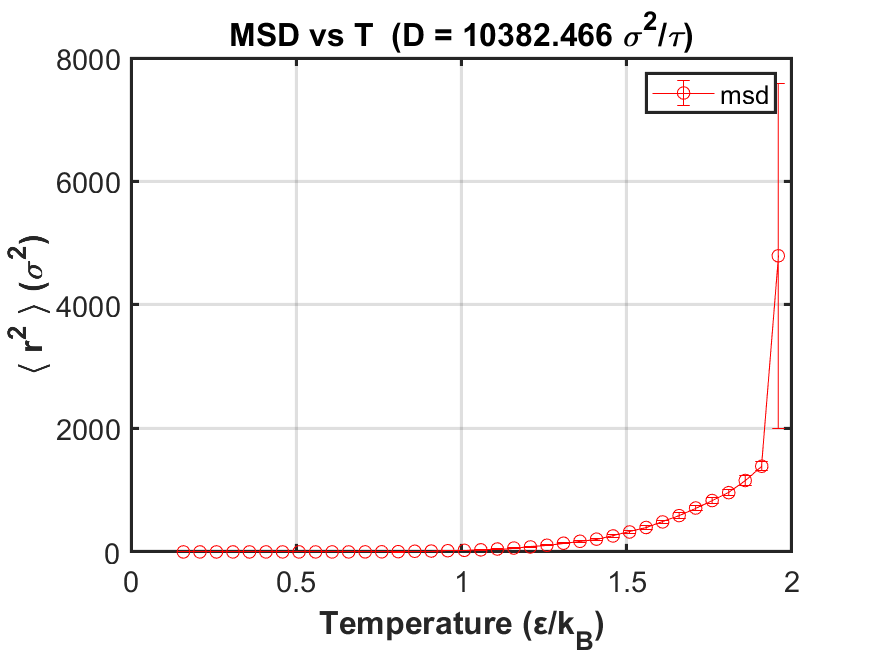
\includegraphics[width=0.7\textwidth]{Fig_msd_T_mean.png}
    \caption{Mean Square Displacement (MSD) as a function of temperature $T^*$. The sharp increase at higher temperatures indicates the transition to a diffusive liquid.}
    \label{fig:msd_vs_temp}
\end{figure}

\subsection{Radial Pair Distribution Function}


The Radial pair distribution function ($g(r)$) is defined as follows:
$$
g(r) = \frac{1}{\rho N}\left\langle\sum_{i=1}^N\sum_{j\neq i}\delta(r-r_{ij})\right\rangle
$$
It represents the probability, relative to an ideal gas, of finding a pair of atoms separated by a distance $r$.

It describes how density varies as a function of distance from a reference particle in a many-body system. In simpler terms, it provides the probability of finding particles at a certain distance $r$ compared to what you would expect in a completely uniform system.
\begin{itemize}
    \item $g(r)=1$ implies that, at distance $r$, particles are distributed at the same density as a random, uniform distribution.
    \item $g(r)>1$ indicates an enhanced probability at distance $r$.
    \item $g(r)<1$ indicates a depleted probability.
\end{itemize}
In solid phases, $g(r)$ shows distinct peaks at specific distances corresponding to the crystal's coordination shells. In the fluid phase, the peaks are broader and less pronounced, reflecting greater disorder.

The evolution of the radial pair distribution function, $g(r)$, provides a clear structural picture of the transition (\textbf{Fig. \ref{fig:gr_all}}).
\begin{itemize}
    \item \textbf{Solid Phase (Fig. \ref{fig:gr_solid}):} At low temperature, the $g(r)$ shows a series of sharp, well-defined peaks, corresponding to the coordination shells of the FCC lattice. The first maximum reaches a value of $g_{max} \approx 6.8$, indicating that the nearest-neighbour shells are virtually undeformed. The oscillations remain well-defined even at larger distances, demonstrating long-range translational order. The extremely sharp minima, at which $g(r)$ falls close to zero, confirm that thermal vibrations are still small compared with the inter-atomic spacing.
    \item \textbf{Melting Phase (Fig. \ref{fig:gr_melting}):} At the transition temperature, the profile is intermediate. The first peak is significantly lower and broader than in the solid phase ($g_{max} \approx 2.8$), indicating increased atomic mobility, yet it remains much more pronounced than in the final liquid phase. 
    \item \textbf{Liquid Phase (Fig. \ref{fig:gr_liquid}):} Well above melting, only a broad first peak remains with a markedly reduced amplitude ($g_{max} \approx 1.7$), followed by a rapid decay to $g(r)=1$, signifying the loss of long-range order.
\end{itemize}

\begin{figure}[h!]
    \centering
    \begin{subfigure}{.7\textwidth}
        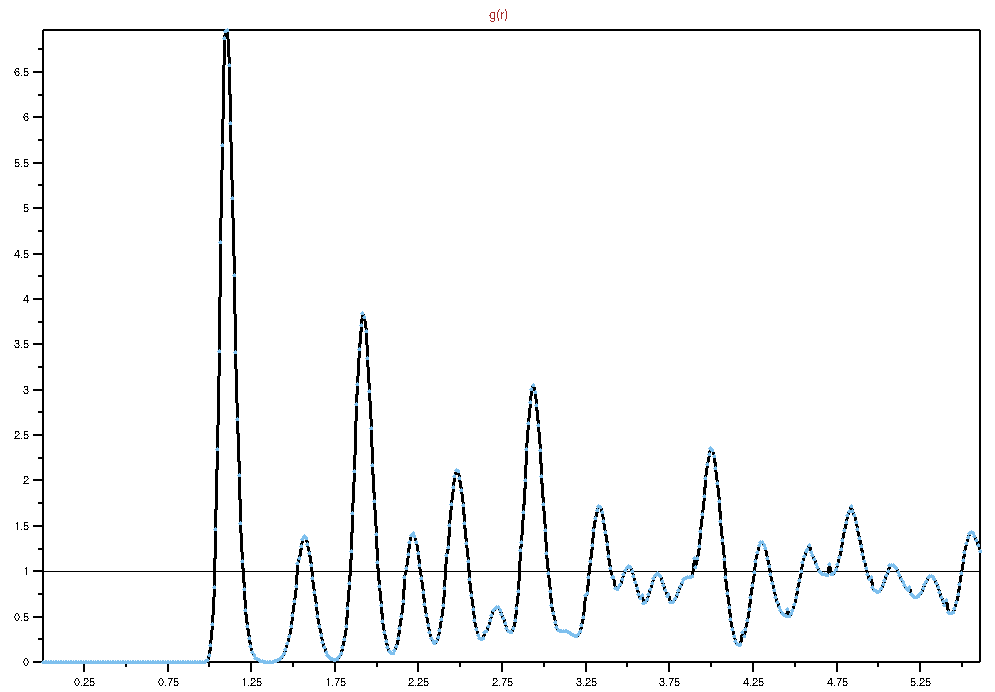
\includegraphics[width=\linewidth]{g(r)_solid.png} 
        \caption{Solid phase \\($T^*=0.3$).}
        \label{fig:gr_solid}
    \end{subfigure}
    \begin{subfigure}{.7\textwidth}
        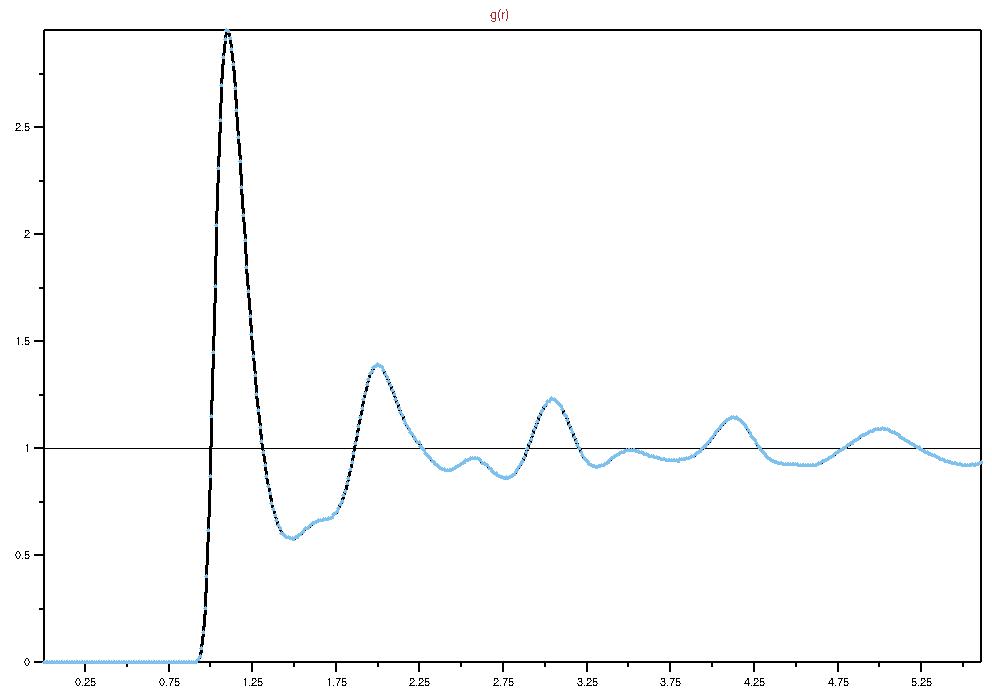
\includegraphics[width=\linewidth]{g(r)_melting.png}
        \caption{Melting transition \\($T^* \approx 0.8$).}
        \label{fig:gr_melting}
    \end{subfigure}
    \begin{subfigure}{.7\textwidth}
        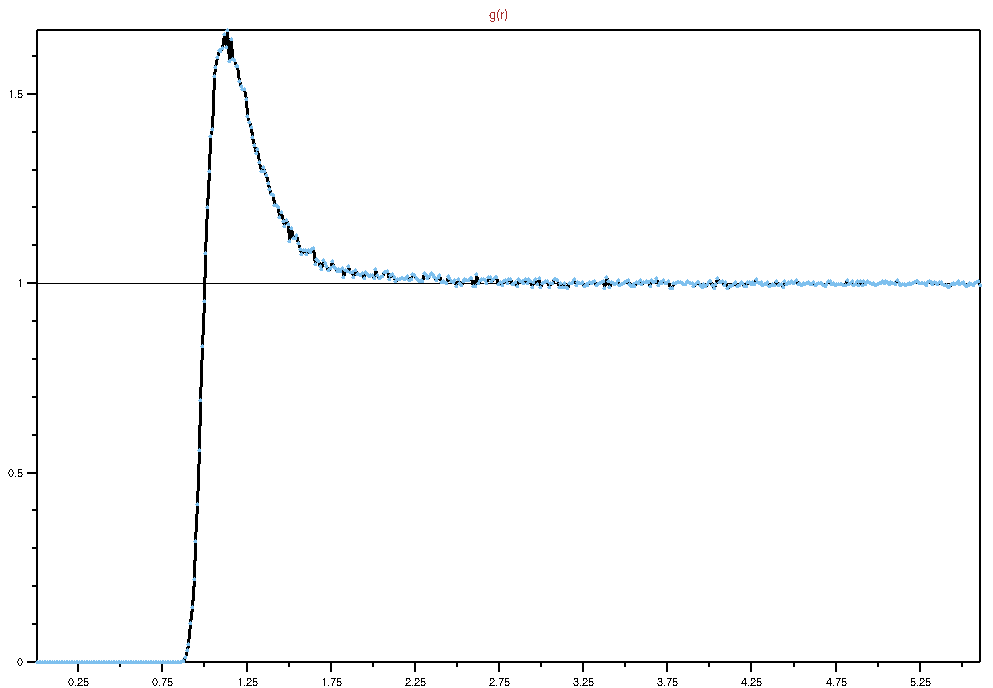
\includegraphics[width=\linewidth]{g(r)_liquid.png} 
        \caption{Liquid phase \\($T^*=2.0$).}
        \label{fig:gr_liquid}
    \end{subfigure}
    \caption{The radial pair distribution function $g(r)$ at different stages, showing the progressive loss of structural order.}
    \label{fig:gr_all}
\end{figure}

\section{Discussion: Kinetic Effects and Superheating}

Our analysis consistently places the melting transition in the range of $T^* \approx 0.80 - 0.85$. However, the accepted thermodynamic melting temperature of the LJ solid at zero pressure is reported in the literature to be significantly lower, at $T_m^{\text{lit}} \approx 0.69\,\epsilon/k_B$ \cite{HansenVerlet}.

This discrepancy is a well-known kinetic artifact in MD simulations: \textbf{superheating}. Due to the finite heating rate, the system does not have enough time to form the critical nuclei of the liquid phase at the true melting point and instead persists in a metastable solid state until a higher temperature. The reverse phenomenon, supercooling, is observed when a liquid is cooled below its freezing point without crystallizing.

To verify the presence of superheating, we repeated the simulation with four different heating ramps, corresponding to total heating durations of $10,000$, $20,000$, $40,000$, and $80,000$ steps. The results, shown in \textbf{Figure \ref{fig:heating_rates}}, clearly demonstrate that the observed melting temperature depends on the heating rate. The fastest ramp exhibits the highest transition temperature, while the slowest ramp shows the lowest. As the heating rate decreases, the observed melting point shifts closer to the true thermodynamic value. This provides direct evidence that our simulations exhibit superheating and that obtaining an accurate estimate of $T_m$ would require even slower heating rates and an extrapolation to a zero-rate limit.

It is important to note that achieving complete equilibration during the temperature ramp is particularly challenging, especially near the phase transition. At these conditions, the relaxation timescales for structural rearrangements are significantly longer due to the formation of critical nuclei and the coexistence of phases. Consequently, the system may not reach a fully equilibrated state at each temperature step during the heating process. Our approach, therefore, focuses on identifying and quantifying kinetic effects such as superheating rather than determining the exact thermodynamic melting point \cite{FrenkelSmit}.

Additionally, the size of the simulated system ($N=4000$ particles) may influence the observed melting behavior. Finite-size effects can impact the nucleation of the liquid phase and the stability of the metastable solid state. Simulations with larger systems are expected to reduce such effects and provide results closer to the thermodynamic limit, as reported in studies of Lennard-Jones systems.


\begin{figure}[htbp]
    \centering
    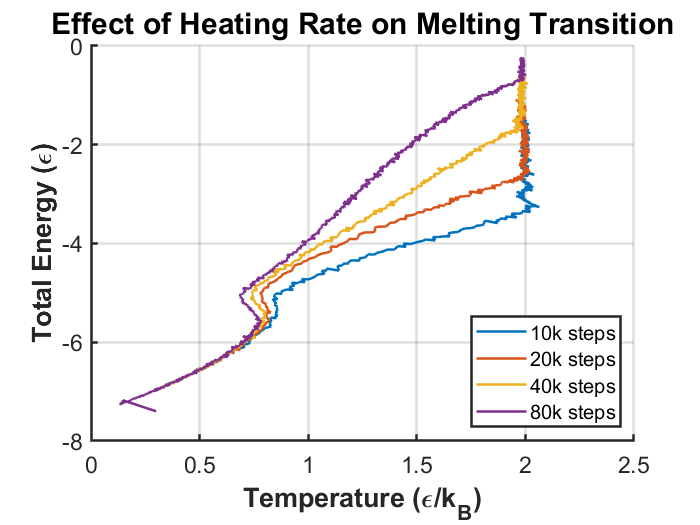
\includegraphics[width=0.8\linewidth]{heating_ramp.png}
    \caption{Total energy as a function of temperature for four different heating rates. As the heating rate decreases, the observed melting transition shifts to lower temperatures, demonstrating the effect of superheating.}
    \label{fig:heating_rates}
\end{figure}

\subsection{Dynamical Hysteresis (MSD)}

The Mean Square Displacement provides a complementary view of the dynamics (\textbf{Figure \ref{fig:hyst_msd}}).
\begin{itemize}
    \item \textbf{Heating (Red Curve):} The MSD is near zero in the solid phase, confirming that atoms are confined. It begins to rise sharply only after the system melts and becomes a diffusive liquid.
    \item \textbf{Cooling (Blue Curve):} The MSD on the cooling path starts at a very high value, as it is a cumulative measure of the total displacement from the simulation's origin. As the system cools, the curve flattens. This flattening signifies a \textbf{dynamical arrest}: the atoms stop diffusing and become trapped in a disordered, glassy configuration. The final high value of the MSD confirms that the system did not return to its original crystalline state.
\end{itemize}

Taken together, these two plots provide definitive evidence of a hysteresis cycle driven by kinetic barriers to nucleation, confirming both superheating on melting and supercooling/vitrification on freezing.

\begin{figure}[h!]
    \centering
    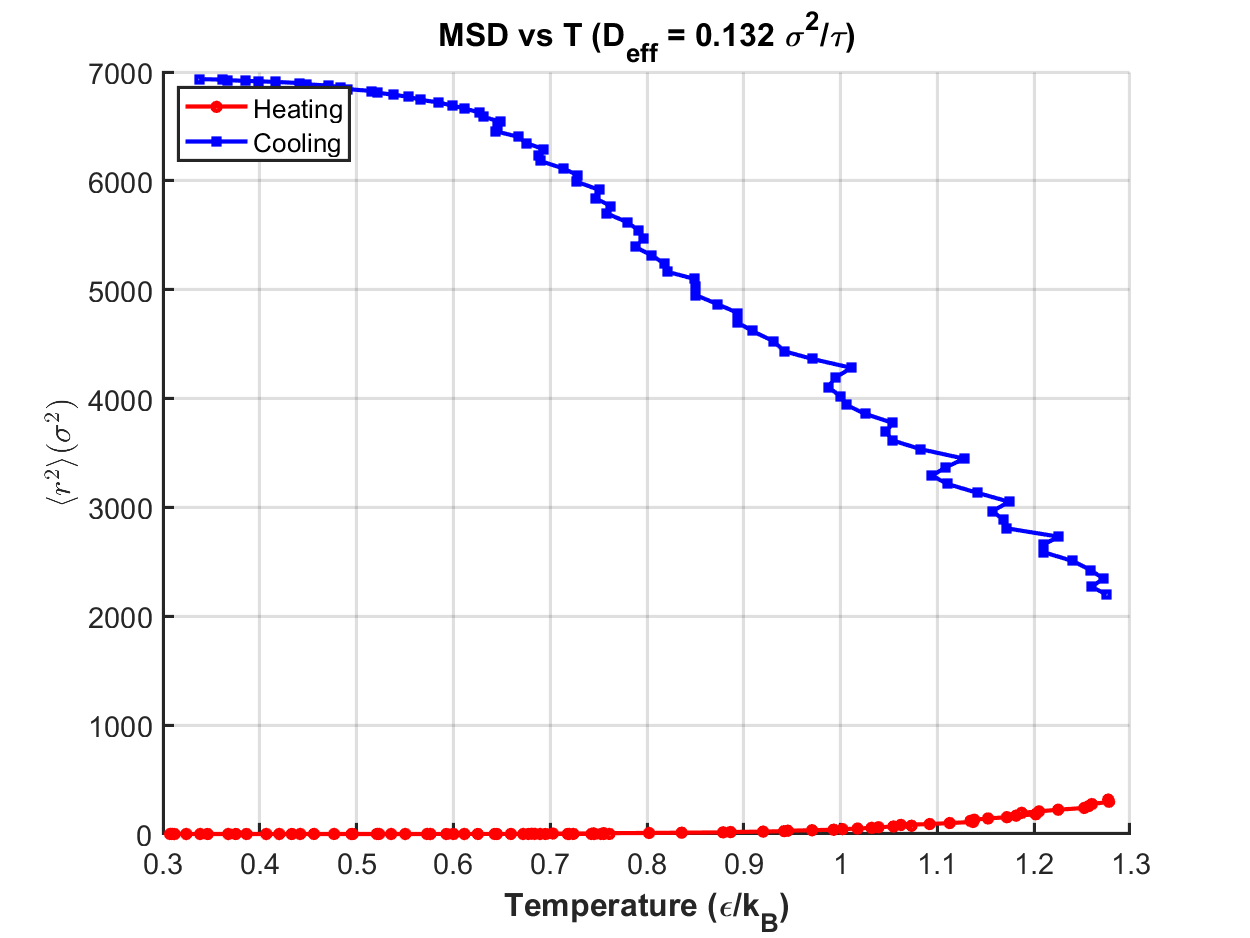
\includegraphics[width=0.8\linewidth]{temp_msd.png}
    \caption{Mean Square Displacement during the hysteresis cycle. The system becomes diffusive (rising MSD) only upon melting and then undergoes dynamical arrest (flattening MSD) upon cooling into a glassy state.}
    \label{fig:hyst_msd}
\end{figure}


\section{Conclusion}

In this study, we successfully simulated the melting of a Lennard-Jones FCC crystal. The analysis of thermodynamic, structural, and dynamical observables provided consistent evidence of a first-order phase transition. Our simulations identified an observed melting temperature of approximately $T_{obs}^* \approx 0.75 - 0.80$.

We have demonstrated that this value does not represent the true thermodynamic melting point but is an overestimate due to the kinetic effect of superheating. The reliability of this result was assessed through two key analyses. First, a systematic study with different heating rates confirmed that the observed melting temperature is rate-dependent, approaching the accepted literature value of $T_m^{\text{lit}} \approx 0.69\,\epsilon/k_B$ only in the limit of an infinitely slow heating rate \cite{HansenVerlet, AgrawalKofke}. Second, a simulation of a full heating-cooling cycle revealed a clear hysteresis loop, visually confirming both superheating during melting and the corresponding phenomenon of supercooling and vitrification upon cooling.

This work underscores the critical importance of accounting for kinetic artifacts in the simulation of phase transitions and illustrates standard methodologies for assessing the reliability of a computationally determined melting point.



\begin{thebibliography}{9}


\bibitem{LAMMPS}
Aidan P. Thompson, H. Metin Aktulga, LAMMPS - a flexible simulation tool for particle-based materials modeling at the atomic, meso, and continuum scales, \textit{Computer Physics Communications.}, \textbf{Volume 271} (February 2022).

\bibitem{VMD}
W. Humphrey, A. Dalke, and K. Schulten, VMD: Visual Molecular Dynamics, \textit{J. Molec. Graphics}, \textbf{14}, 33-38 (1996).

\bibitem{HansenVerlet}
J.-P. Hansen and L. Verlet, Phase Transitions of the Lennard-Jones System, \textit{Phys. Rev.}, \textbf{184}, 151 (1969).

\bibitem{Nose}
S. Nosé, A molecular dynamics method for simulations in the canonical ensemble, \textit{Mol. Phys.}, \textbf{52}, 255-268 (1984).

\bibitem{Hoover}
W. G. Hoover, Canonical dynamics: Equilibrium phase-space distributions, \textit{Phys. Rev. A}, \textbf{31}, 1695-1697 (1985).

\bibitem{AllenTildesley}
M. P. Allen and D. J. Tildesley, \textit{Computer Simulation of Liquids}, 2nd ed. (Oxford University Press, 2017).

\bibitem{AgrawalKofke}
R. Agrawal and D. A. Kofke, Thermodynamic and structural properties of the high density hard-core fluid and solid, \textit{Mol. Phys.}, \textbf{85}, 43-59 (1995).


\bibitem{FrenkelSmit}
D. Frenkel and B. Smit, \textit{Understanding Molecular Simulation: From Algorithms to Applications}, 2nd ed. (Academic Press, 2002).

\end{thebibliography}

\end{document}
